\documentclass{standalone}
\usepackage{tikz}
\usetikzlibrary{arrows.meta, positioning, shapes.geometric, calc,patterns}

\begin{document}
	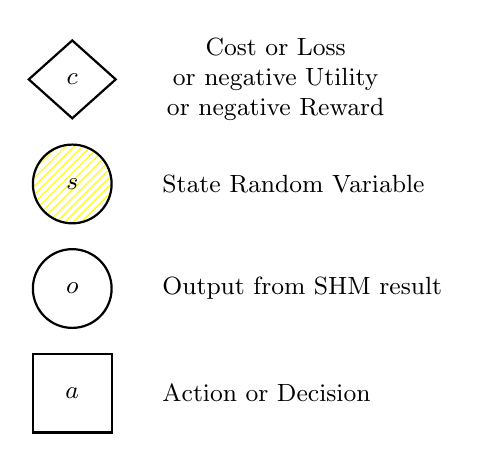
\begin{tikzpicture}[
		node distance=2cm and 1.5cm,
		every node/.style={draw, minimum size=10mm, font=\small},
		cost/.style={diamond, aspect=2, fill=white},
		shaded/.style={circle,pattern=north east lines, pattern color=yellow},
		obs/.style={circle, fill=white},
		action/.style={rectangle, fill=white},
		->, >=Stealth, thick, black
		]
		
		% Denote 
		\node[cost] at (-7,0) (costnode) {$c$};
		\node[draw = white,right= of costnode,xshift = -10mm,align=center]  {Cost or Loss \\ or negative Utility \\or negative Reward};
		\node[shaded, below = of costnode, yshift = 17mm] (statenode) {$s$};
		\node[draw = white, right = of statenode,xshift = -10mm,align = center] {State Random Variable};
		\node[obs, below= of statenode,yshift = 17mm]  (obsnode) {$o$};
		\node[draw = white, right = of obsnode,xshift = -10mm,align = center]  {Output from SHM result};
		\node[action,below = of obsnode,yshift = 17mm]  (actionnode) {$a$};
		\node[draw = white, right = of actionnode,xshift = -10mm, align=center] {Action or Decision };
		
	\end{tikzpicture}
\end{document}
